\chapter[The Triple Pendulum]{The Triple Pendulum:\\Coupling, Release and Control}
\label{ch:triple_pendulum}
\index{Wrist release}
\index{Wrist cock}
\index{Whip effect}
\index{Triple pendulum}
\index{Sequential unlocking}
\index{Mass matrix coupling}
\index{Kinetic chain}
\index{Energy redistribution}
\index{Coriolis whip}
\raggedbottom

\begin{laymansbox}{What an Additional Joint Lets Us Investigate}{context:triple_pendulum_motivation}
A moving arm and club exchange energy through their connections. Muscles can add or absorb mechanical energy, while joint forces redirect motion and transfer power between bodies. An additional joint gives the system another way to change its shape and redistribute its motion. It does not guarantee a faster club, a particular release sequence or less muscular work.

The useful question is therefore specific: for the same bodies, initial state, admissible inputs and task, how does allowing an additional relative rotation change the attainable club motion? This chapter builds the mechanics needed to answer that question. A two-link arm--club model already includes a wrist hinge. Here the third link resolves an upper arm and forearm separately; it is a choice of resolution, not a universal minimum for explaining golf speed.
\end{laymansbox}

Our investigation connects four quantities that are often conflated: joint torque, segment power, angular velocity and clubhead velocity. A large club angular velocity need not imply large contemporaneous wrist power. Conversely, small net wrist work does not establish that the wrist is uncontrolled or mechanically unimportant. The configuration and the history of applied forces determine how those quantities relate.

\section{The Triple Pendulum Model}
\label{sec:triple_pendulum_setup}
\begin{definition}{Three Rigid Links and Three Relative Angles}{triple_pendulum}
Use a fixed shoulder pivot and three ideal planar revolute joints. Link 1 represents an upper arm, link 2 a forearm-and-hand aggregate, and link 3 a rigid club. Each link has length $L_i$, positive mass $m_i$, COM distance $c_i$ from its proximal joint, and positive planar rotational inertia $I_i$ about its own center of mass. These are independent specified body properties. An inertia measured about a proximal joint must first be converted using $I_{i,\mathrm{joint}}=I_i+m_i c_i^2$; adding that offset again would double-count it.

The angle $q_1$ is measured counterclockwise from downward vertical. The angles $q_2$ and $q_3$ are measured from the preceding link. Thus $q_2=0$ means aligned links, whereas $q_2=90^\circ$ means a right angle. The absolute orientations are
\[
\theta_1=q_1,\qquad \theta_2=q_1+q_2,\qquad
\theta_3=q_1+q_2+q_3.
\]
The configuration space of these ideal unrestricted hinges is a three-torus; computations use local or unwrapped radian coordinates in $\mathbb R^3$. Anatomical limits would restrict this domain. Relative joint rates $v=\dot q$ differ from absolute segment rates $\omega_i=\dot\theta_i$.
\end{definition}

\subsection{Understanding the Three Segments}
\label{inplain:triple_pendulum_segments}
\label{laymans:inplain:triple_pendulum_segments}
The shoulder is fixed in this example. There is no rotating torso, moving pelvis, second arm, shaft bending or ground-contact model hidden inside its parameters. The grip hinge is an ideal planar coordinate, not a measurement of anatomical wrist extension, radial deviation or forearm rotation. In particular, it cannot predict three-dimensional clubface orientation. Those features require additional bodies, coordinates and constraints.

Mass alone does not order rotational inertia: the distance of mass from the reference axis matters. A long light club can have greater inertia about its grip than a heavier compact body about another axis. Nor does an inertia ranking establish which segment must move fastest in a coupled chain. The relevant kinetic energy includes COM motion and all absolute angular velocities.

\begin{figure}[H]
\centering
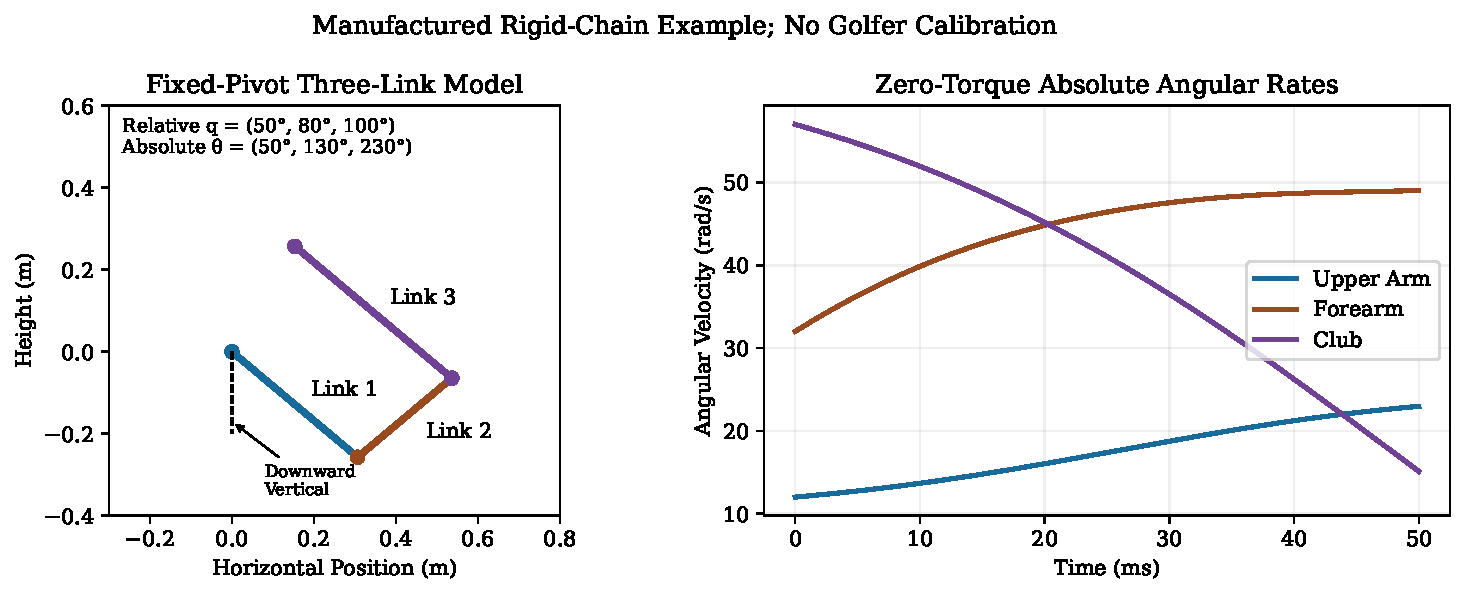
\includegraphics[width=\linewidth]{figures/triple_pendulum_verified.pdf}
\caption{Three-Link Geometry and an Unforced Continuation From the Declared Initial State. Absolute Club Angular Velocity Decreases in This Example; an Additional Joint Does Not Guarantee Distal Acceleration. These Are Manufactured Dynamics, Not a Measured Golf Swing.}
\label{fig:triple_pendulum_diagram}
\end{figure}

Write the direction of a link as $e(\theta)=(\sin\theta,-\cos\theta)^T$. The COM position and its Jacobian are
\[
r_i=\sum_{k<i}L_k e(\theta_k)+c_i e(\theta_i),\qquad
J_i=\frac{\partial r_i}{\partial q}.
\]
For $j\le i$, column $j$ of $J_i$ contains $\sum_{k=j}^{i-1}L_k e'(\theta_k)+c_i e'(\theta_i)$; later columns are zero. Let $s_i$ be the vector with its first $i$ entries equal to one and all later entries zero. Then $\dot r_i=J_i v$ and $\omega_i=s_i^T v$. This construction fixes the meaning of every subsequent term.

\section{Equations of Motion for the Triple Pendulum}
\label{sec:triple_pendulum_eom}
\label{thm:theorem:triple_pendulum_dynamics}
\begin{definition}{Kinetic Energy, Gravity and Applied Torque}{theorem:triple_pendulum_dynamics}
For the rigid, frictionless chain,
\[
T=\frac12\sum_i\left(m_i\lVert J_i v\rVert^2+I_i(s_i^T v)^2\right)
 =\frac12 v^T M(q)v,\qquad V=\sum_i m_i g_0(r_i)_y,
\]
where $g_0=9.81\ \mathrm{m/s^2}$ and upward height is positive. Define $g(q)=\nabla_q V$. Lagrange's equations give
\begin{equation}
M(q)\ddot q+c(q,v)+g(q)=\tau.
\label{eq:triple_pendulum_eom}
\end{equation}
The vector $c$ contains the velocity-dependent inertial terms; it is not itself a Coriolis matrix. The input $\tau_i$ is the net applied joint couple conjugate to relative rate $v_i$, so its mechanical power is $\tau_i v_i$. It is not an individual muscle force or neural excitation.
\end{definition}

To verify the gravity convention, set $h_1=m_1c_1+(m_2+m_3)L_1$, $h_2=m_2c_2+m_3L_2$ and $h_3=m_3c_3$. Then $V=-g_0\sum_i h_i\cos\theta_i$ and
\[
g=g_0\begin{bmatrix}
h_1\sin\theta_1+h_2\sin\theta_2+h_3\sin\theta_3\\
h_2\sin\theta_2+h_3\sin\theta_3\\h_3\sin\theta_3
\end{bmatrix}.
\]
At rest with every link pointing down, gravity torque is zero. Displacing the chain slightly requires a holding torque with the sign of this potential gradient; the unforced acceleration uses its negative after solving through $M$.

\section{The Mass Matrix: Understanding Coupling}
\label{sec:triple_pendulum_mass_matrix}
\begin{definition}{Complete Three-Link Inertia}{triple_pendulum_mass_matrix}
The COM construction yields
\begin{equation}
M=\sum_i\left(m_i J_i^T J_i+I_i s_i s_i^T\right)
=\begin{bmatrix}M_{11}&M_{12}&M_{13}\\M_{12}&M_{22}&M_{23}\\M_{13}&M_{23}&M_{33}\end{bmatrix}.
\label{eq:triple_mass_matrix_structure}
\end{equation}
For compact complete entries, define
\[
\begin{aligned}
a&=I_1+m_1c_1^2+(m_2+m_3)L_1^2,\\
b&=I_2+m_2c_2^2+m_3L_2^2,\qquad d=I_3+m_3c_3^2,\\
\alpha&=m_2L_1c_2+m_3L_1L_2,\quad
\beta=m_3L_1c_3,\quad \gamma=m_3L_2c_3.
\end{aligned}
\]
Every constant has units $\mathrm{kg\,m^2}$. The entries are
\[
\begin{aligned}
M_{11}&=a+b+d+2\alpha\cos q_2+2\beta\cos(q_2+q_3)+2\gamma\cos q_3,\\
M_{22}&=b+d+2\gamma\cos q_3,\qquad M_{33}=d,\\
M_{12}&=b+d+\alpha\cos q_2+\beta\cos(q_2+q_3)+2\gamma\cos q_3,\\
M_{13}&=d+\beta\cos(q_2+q_3)+\gamma\cos q_3,\\
M_{23}&=d+\gamma\cos q_3.
\end{aligned}
\]
In particular, $M_{11}$ includes all three COM inertias, and both $M_{22}$ and $M_{12}$ include $I_2+I_3$. Their presence follows from the absolute angular rates. Omitting them requires an explicitly justified point-mass approximation, not merely the observation that a club is light. A club generally does not have $c_3=L_3/2$; that is only an assumption in the manufactured examples below.
\end{definition}

For any nonzero $v$, the angular contribution $\sum_i I_i(s_i^T v)^2$ is positive because the three $s_i$ span the velocity space. Thus the declared model has a symmetric positive-definite $M$ at every configuration. This property survives a task-Jacobian singularity: the tip may lose an instantaneous motion direction even while the joint-space inertia remains invertible.

\subsection{What the Mass Matrix Entries Mean}
\label{inplain:mass_matrix_meaning}
\label{laymans:inplain:mass_matrix_meaning}
At a fixed state, an incremental applied torque produces $\delta\ddot q=M^{-1}\delta\tau$. The inverse, rather than an isolated entry of $M$, determines acceleration response. Off-diagonal entries describe inertial coupling in the stated coordinates; they do not guarantee simultaneous motion, a universal ordering such as $M_{13}>M_{12}$, or diagonal dominance. Torques or constraints can hold selected coordinates fixed while others move.

The diagonal $M_{ii}$ describes the inertia for accelerating coordinate $i$ while all other accelerations are held zero, with the necessary reaction torques supplied. If the other joints instead respond freely to an incremental torque only at $i$, the apparent inertia is
\[
I_{i,\mathrm{free}}=\frac{1}{(M^{-1})_{ii}}
=M_{ii}-M_{ir}M_{rr}^{-1}M_{ri},
\]
the Schur complement of the remaining coordinates $r$. These are different experiments. Neither quantity alone measures anatomical strength, energetic efficiency or control precision.

\begin{example}{A Computed Matrix and Its Inverse}{triple_pendulum_mass_numerical}
Use $L=(0.4,0.3,0.5)\ \mathrm m$, $m=(2,0.5,0.2)\ \mathrm{kg}$, $I=(0.05,0.01,0.01)\ \mathrm{kg\,m^2}$ and $c_i=L_i/2$. This is a manufactured short-club chain, not calibrated adult-driver anthropometry. At $q=(50,90,100)^\circ$,
\begin{equation}
M\simeq\begin{bmatrix}
0.259148&0.036844&0.000199\\
0.036844&0.056541&0.019895\\
0.000199&0.019895&0.022500
\end{bmatrix}\ \mathrm{kg\,m^2}.
\label{eq:triple_mass_numerical}
\end{equation}
The unrounded matrix has eigenvalues approximately $0.012310$, $0.060183$ and $0.265696\ \mathrm{kg\,m^2}$. Its computed inverse is
\begin{equation}
M^{-1}\simeq\begin{bmatrix}
4.45187&-4.19125&3.66665\\
-4.19125&29.62083&-26.15467\\
3.66665&-26.15467&67.53886
\end{bmatrix}\ (\mathrm{kg\,m^2})^{-1}.
\label{eq:triple_mass_inverse_numerical}
\end{equation}
An incremental $1\ \mathrm{N\,m}$ at joint 3 therefore changes the acceleration vector by approximately $(3.67,-26.15,67.54)\ \mathrm{rad/s^2}$. The free apparent inertia at that coordinate is $0.01481\ \mathrm{kg\,m^2}$, compared with $M_{33}=0.02250$ when the other accelerations are fixed. A large response can amplify disturbances as well as useful inputs; it does not prove high precision.
\end{example}

\section{Coriolis Terms in the Triple Pendulum}
\label{sec:triple_pendulum_coriolis}
\subsection{The Velocity-Dependent Terms and Their Signs}
\label{inplain:triple_coriolis_complexity}
\label{laymans:inplain:triple_coriolis_complexity}
The complete Christoffel expression is
\begin{equation}
c_i=\sum_{j,k}\frac12\left(
\frac{\partial M_{ij}}{\partial q_k}
+\frac{\partial M_{ik}}{\partial q_j}
-\frac{\partial M_{jk}}{\partial q_i}\right)v_jv_k.
\label{eq:coriolis_general_form}
\end{equation}
Keeping only $\sum_{j,k}(\partial M_{ij}/\partial q_k)v_jv_k$ omits the kinetic-energy gradient. A useful independent check is $v^T c=\tfrac12v^T\dot Mv$. Multiplying the equation of motion by $v^T$ then gives $\dot T+\dot V=\tau^T v$. Velocity-dependent inertia can redistribute motion while satisfying this energy balance; it is not an additional energy source.

For the distal coordinate the cancellations simplify considerably:
\begin{equation}
c_3=\beta\sin(q_2+q_3)v_1^2
+\gamma\sin q_3(v_1+v_2)^2.
\label{eq:coriolis_club_example}
\end{equation}
There is no $\partial M_{23}/\partial q_2$ contribution because $M_{23}=d+\gamma\cos q_3$ is independent of $q_2$. Also, $v_3$ cancels from this particular generalized component, although it remains in the other components and therefore can affect $\ddot q_3$ through the coupled solve. Neither $c_3$ nor $-c_3/M_{33}$ alone is the freely responding club acceleration.

\begin{example}{A Signed Inertial Term}{triple_coriolis_whip}
At $q=(50,80,100)^\circ$ and $v=(12,20,25)\ \mathrm{rad/s}$ with the preceding parameters, $\beta=0.02$ and $\gamma=0.015\ \mathrm{kg\,m^2}$. Therefore
\begin{equation}
c_3=0.02\sin180^\circ(12)^2+0.015\sin100^\circ(32)^2
\simeq15.127\ \mathrm{N\,m}.
\label{eq:coriolis_club_magnitude}
\end{equation}
This term sits on the left of the equation of motion. It is not a measured wrist-muscle torque or proof of distal acceleration. Reversing both relative configuration angles reverses its sign at fixed rates; at straight alignment it vanishes. In the full unforced example below, the club's absolute angular rate decreases despite its initially large value.
\end{example}

\section{The Whip Effect: What Constraint Release Changes}
\label{sec:whip_effect}
\label{princ:principle:whip_effect}
\begin{definition}{An Ideal Release Event}{whip_effect}
Suppose a mechanical lock holds $q_3=\bar q_3$ with $v_3=0$. With $A=(0,0,1)$, its equations are
\[
\begin{bmatrix}M&-A^T\\A&0\end{bmatrix}
\begin{bmatrix}\ddot q\\\lambda\end{bmatrix}
=\begin{bmatrix}\tau-c-g\\0\end{bmatrix}.
\]
The multiplier supplies the joint reaction required to maintain the lock. Because $Av=0$, its power $\lambda^T Av$ is zero. This is a stationary ideal constraint; a driven constraint can do work.

Remove the lock with no impulse and no instantaneous change in potential or body properties. Position and velocity are continuous: $q^+=q^-$ and $v^+=v^-$. Mechanical energy is consequently continuous. Acceleration can jump when the reaction is removed. There is no instantaneous inheritance of another body's momentum and no injection of energy by the removal itself.
\end{definition}

\subsection{Why the State at Release Matters}
\label{inplain:sequential_unlocking_why}
\label{laymans:inplain:sequential_unlocking_why}
The state reached before release reflects all earlier inputs and constraints. Changing a holding interval can change that state, the subsequent force transmission and the timing of a useful tip trajectory. That provides a mechanism by which release timing can matter. It does not imply that a later release always improves speed or that shoulder, elbow and wrist must unlock at universal times.

For the manufactured chain, use $q=(50,80,100)^\circ$ and the compatible locked rate $v=(12,20,0)\ \mathrm{rad/s}$ with zero applied joint torques. Immediately before removal,
\[
\ddot q^-\simeq(199.109,-308.438,0)^T\ \mathrm{rad/s^2},\qquad
\lambda\simeq8.594\ \mathrm{N\,m}.
\]
Immediately afterward the same state gives
\[
\ddot q^+\simeq(158.666,-65.564,-596.883)^T\ \mathrm{rad/s^2}.
\]
The negative relative wrist acceleration is a computed result, not a release rule. The change in acceleration satisfies $M(\ddot q^- -\ddot q^+)=A^T\lambda$. Both sides of the event have the same energy. In contrast, suddenly imposing a lock on an incompatible nonzero $v_3$ generally requires an impulse and a separately specified impact law; that is a different event.

\section{Wrist Cock and Release as a Constraint Mechanism}
\label{sec:wrist_cock_release}
\label{ex:wrist_cock_timing}
\begin{definition}{A Pose, a Lock and a Spring Are Different Models}{wrist_cock_release}
A bent wrist pose by itself specifies neither a force nor stored energy. In these relative coordinates, a fixed wrist angle is $q_3=\bar q_3$. Fixing the sum of the second and third relative angles would instead fix the club orientation relative to the upper arm, a different constraint. Neither condition should be inferred merely from a projected video angle.

An ideal lock enforces a geometric condition. An active joint controller uses torque to maintain an approximate pose. A passive elastic joint supplies a configuration-dependent torque and stores recoverable energy. A viscoelastic joint also depends on deformation history and dissipates energy. These mechanisms can produce similar-looking motion while having different power and control requirements.
\end{definition}

\subsection{Wrist Cock and Recoverable Energy}
\label{inplain:wrist_cock_energy}
\label{laymans:inplain:wrist_cock_energy}
For a declared linear torsional spring with natural angle $q_{3,0}$,
\[
U_s=\frac12 k(q_3-q_{3,0})^2,\qquad
\tau_s=-k(q_3-q_{3,0}).
\]
With parallel damping $\tau_d=-b v_3$, the rigid-chain balance becomes
\[
\frac{d}{dt}(T+V+U_s)=\tau_{\mathrm{active}}^T v-bv_3^2,
\qquad b\ge0.
\]
Recoil can supply power when $U_s$ decreases. Estimating how much a human wrist supplies requires measured torque--angle behavior, its natural configuration, rate/history effects and the actual multi-axis motion. A cock angle or a generic tendon stiffness is insufficient to establish a universal 5--10 J store or its fraction of club energy.

An actively held posture can have zero joint mechanical power while muscles consume metabolic energy or exchange energy internally. Net joint power also cannot identify co-contraction. This is why mechanical work, motor commands, tissue loading and subjective effort must remain separate in the explanation. The muscle-force and fascia chapters develop the actuator and material states needed to connect them.

\section{Triple Pendulum ZTCF Family: A Computed Counterfactual}
\label{sec:triple_pendulum_ztcf}
\label{ex:triple_pendulum_ztcf_example}
Setting the declared generalized input to zero gives
\begin{equation}
\dot q=v,\qquad \dot v=-M(q)^{-1}\bigl(c(q,v)+g(q)\bigr).
\label{eq:triple_ztcf_ode}
\end{equation}
Here the model is frictionless and has no spring, muscle-activation or material-memory state. Gravity remains. If those states or passive forces are added, they must remain in the appropriate counterfactual equations; zero neural excitation would not mean zero muscle force. A pointwise zero-torque acceleration and a forward trajectory that keeps torque zero for 50 ms answer different questions. The trajectory evolves through states different from any actively controlled continuation.

Use the preceding manufactured body parameters with $q(0)=(50,80,100)^\circ$ and $v(0)=(12,20,25)\ \mathrm{rad/s}$. Convert initial angles to radians before integration. The initial acceleration is approximately $(131.936,809.896,-1371.119)\ \mathrm{rad/s^2}$, computed from the complete equations rather than assigned independently.


\begin{table}[H]
\centering
\caption{Manufactured Zero-Torque Continuation: Absolute Rates and Tip Speed}
\begin{tabular}{rrrrr}
\toprule
$t$ (ms) & $\omega_1$ (rad/s) & $\omega_2$ (rad/s) & $\omega_3$ (rad/s) & Tip (m/s) \\
\midrule
0 & 12.000 & 32.000 & 57.000 & 23.976 \\
25 & 17.382 & 46.411 & 41.051 & 12.937 \\
50 & 22.961 & 49.001 & 15.120 & 7.924 \\
\bottomrule
\end{tabular}
\end{table}


The angle vectors at 25 and 50 ms are approximately $(70.582,117.600,113.367)^\circ$ and $(99.942,157.321,85.308)^\circ$. At 50 ms the relative rates are $(22.961,26.041,-33.881)\ \mathrm{rad/s}$; the club's absolute rate is their sum, $15.120\ \mathrm{rad/s}$. Confusing $v_3$ with $\omega_3$ would reverse the interpretation of its rotation.

The reproducible calculation uses DOP853 with relative tolerance $10^{-10}$, absolute tolerance $10^{-12}$ and maximum step 1 ms, sampled every 0.1 ms. Tightening those tolerances to $10^{-12}$ and $10^{-13}$ and halving the maximum step changes each state component by less than $10^{-8}$ in its own radian or radian-per-second units. The variation of $T+V$ stays below $10^{-7}$ J. COM-Jacobian inertia is independently compared with the printed closed entries, and recursive Newton--Euler bias with the Christoffel expression. These checks verify this manufactured calculation; they do not validate it as a golfer.

The tip speed falls from 23.976 to 7.924 m/s in this interval. The club kinetic energy falls from 31.241 to 5.419 J, while upper-arm kinetic energy rises from 9.360 to 34.268 J. This is a counterexample to inevitable proximal-to-distal energy concentration. Other initial states and torque histories can produce distal acceleration; the equations specify how to test them. Reversibility of ideal mechanics does not supply a universal preferred direction of energy transfer.

\subsection{Drift, Available Control and the Task Output}
\label{constraint:triple_dcr_blowup}
The six-state dynamics are control-affine for this torque-input model:
\[
\dot x=f(x)+G(x)\tau,\qquad
f=\begin{bmatrix}v\\-M^{-1}(c+g)\end{bmatrix},\qquad
G=\begin{bmatrix}0\\M^{-1}\end{bmatrix}.
\]
Adding a coordinate does not automatically increase a drift-to-control ratio. The ratio requires a stated output or state metric, input units, admissible torque set and regularization scale. Comparing $f$ with an unspecified control vector conflates available control capacity with the particular torque a golfer happened to apply. A large instantaneous drift contribution cannot establish negligible future control authority or explain neuromuscular effort by itself.

For the rigid tip position $y=r_{\mathrm{tip}}(q)$, where $c_3$ is replaced by $L_3$ in the COM-position construction,
\[
\dot y=J_{\mathrm{tip}}v,\qquad
\ddot y=-J_{\mathrm{tip}}M^{-1}(c+g)+\dot J_{\mathrm{tip}}v
+J_{\mathrm{tip}}M^{-1}\tau.
\]
The geometric acceleration $\dot J_{\mathrm{tip}}v$ matters as well as joint acceleration. Speed, direction, strike location and three-dimensional face orientation are distinct task quantities. This planar model represents only the first two and a planar tip location. It cannot justify claims about minimal clubface-control effort.

A useful comparison propagates a bounded torque perturbation over a specified time interval and measures its effect on the chosen output, with identical starting state and mechanics. If the endpoint is a ball-contact event, changing the trajectory also changes contact time; evaluate the event consistently. Sensitivity to a joint angle may amplify both intended corrections and sensor or execution error. High sensitivity is therefore not synonymous with precision or easy control.

\section{Comparison: Double vs. Triple Pendulum}
\label{sec:double_vs_triple_pendulum}
\label{ex:dcr_double_vs_triple}
The comparison must specify what the two-link model represents. An upper-arm/forearm chain has no club. An arm/club chain has a wrist hinge but lumps arm shape. A model of torso, arm and club has three segments but resolves different anatomy from this chapter. Counting links does not make these models interchangeable.

A controlled reduction of our model locks $q_3=\bar q_3$ and writes
\[
q=N z+\bar q,\qquad
N=\begin{bmatrix}1&0\\0&1\\0&0\end{bmatrix},\qquad
\bar q=(0,0,\bar q_3)^T.
\]
The reduced inertia is $M_r=N^T M N$, with projected bias, gravity and input, and $\dot q=N\dot z$. This preserves the full mass distribution and its kinetic energy. Deleting the club mass or its rotational inertia is not the same reduction. For a different locked coordinate, use its corresponding embedding.

Allowing the third coordinate enlarges the kinematic possibilities. An optimization over a truly larger feasible set cannot reduce the optimum only if every previous trajectory remains feasible, the objective is unchanged, and sufficient admissible torque can reproduce the old lock. Removing a mechanical lock while keeping tight torque bounds need not satisfy that inclusion. A free joint is not an actuator with unlimited holding capacity.

Comparisons should therefore match initial energy and state mapping, body parameters, input and power limits, duration or contact event, and task objective. Report both attainable speed and strike constraints. A universal percentage improvement, fixed mph table or DCR increase cannot be deduced from link count.

\section{Energy Redistribution in the Triple Pendulum}
\label{sec:triple_energy_redistribution}
\label{princ:principle:triple_energy_flow}
\begin{definition}{Segment Energy and Joint Power}{triple_energy_flow}
For segment $i$,
\[
T_i=\frac12m_i\lVert J_i v\rVert^2+\frac12 I_i\omega_i^2,
\qquad \omega_i=\sum_{j\le i}v_j.
\]
Using only $\tfrac12 I_i v_i^2$ omits COM translation and substitutes relative for absolute rotation. The correct segment energies sum to $T$; coordinate cross terms in $\tfrac12v^T Mv$ are not additional stores to assign independently to bodies.
\end{definition}

At an ideal joint, the connected bodies share the velocity $v_P$ of the joint point. A reaction force $F$ can supply power $F\cdot v_P$ to one body and $-F\cdot v_P$ to the other. These powers cancel for the complete chain but can substantially change individual segment energies. Equal and opposite joint couples have total power $\tau_i(\omega_i-\omega_{i-1})=\tau_i v_i$, with the fixed base rate zero. A joint force can thus transfer substantial power to the club while the local wrist couple also adds or absorbs power. These contributions are compatible, not competing descriptions of a single quantity.

To identify a particular transfer, compute each body's external and intersegment force and couple power and include gravitational and elastic terms in the chosen balance. A sequence of angular-speed peaks alone does not identify the transfer path, amount of work or actuator responsible. Nor does one body's decrease in rotational kinetic energy prove its muscles actively brake to accelerate another body.

\subsection{When a Distal Segment Can Move Faster}
\label{inplain:distal_faster_explanation}
\label{laymans:inplain:distal_faster_explanation}
For a single rotation with an identified rotational energy $E_{\mathrm{rot}}$,
\begin{equation}
|\omega|=\sqrt{\frac{2E_{\mathrm{rot}}}{I}}.
\label{eq:energy_velocity_relation}
\end{equation}
This explains how a smaller inertia can support a larger rate at the same allocated rotational energy. In a moving chain, however, that allocation is an outcome of dynamics, and total segment energy also includes translation. Neither the equal-energy premise nor monotonic distal acceleration follows from the formula. Clubhead linear speed further depends on the vector sum of all upstream velocity contributions.

\subsection{What Golf Research Adds}
Sprigings and Mackenzie used an optimized planar torso--arm--club model with bounded muscle-torque generators to compare release strategies. Their reported advantage from delaying release was modest, and active wrist torque after release was advantageous. They also reported substantial power transfer into the club through wrist-joint forces. This model result illustrates why transferred power and local actuator power must be assessed together; it does not validate our upper-arm/forearm/club parameters or prescribe an individual golfer's release time. \citep{SprigingsMackenzie2002Release}

Nesbit's motion-driven three-dimensional analysis examined 85 amateur golfers using a full-body model and flexible club. The study reported marked individual differences and identified wrist motion, hand trajectory and work as relevant to club motion. Its modeled forces and torques depend on measured kinematics and mechanical assumptions; they are not direct measurements of separate muscle forces or the result of randomly assigning release strategies. Its richer model also exposes quantities that a planar hinge cannot resolve, including clubface orientation. \citep{Nesbit2005}

The common lesson is methodological. First define the mechanical system and power ports. Then ask which observed quantities constrain it, which counterfactuals it can support, and which intervention would distinguish alternative explanations. A passive power-transfer pathway does not make the whole golfer passive. Conversely, active control can exploit coupled dynamics without supplying all of a distal segment's instantaneous power locally.

\section{Summary: The Triple Pendulum and the Kinetic Chain}
\label{sec:triple_pendulum_summary}
\label{princ:principle:triple_pendulum_key_takeaways}
Three links let us resolve an additional relative motion. A consistent model connects mass distribution to coupled acceleration, joint forces to segment power, torque to mechanical work, and the resulting configuration and rates to the club's task-space motion. Release changes an admissible motion or a force law; ideal impulse-free removal preserves the instantaneous state and energy. Whether subsequent motion helps the strike remains a question for the specified state, inputs and task.

The investigation should track preparation, energy supply, timing, material storage, feedback and strike constraints together. None is reducible to a count of links or an instantaneous drift ratio. The next step toward a golfer can add a moving base, three-dimensional wrist and shoulder motion, both arms, flexible tissues and contact. A spine connecting pelvis to shoulders is a serial connection; closed loops arise when an additional path reconnects bodies, as when both hands couple the arms through a shared club. The topology and constraint forces must be modeled explicitly.



\begin{exercises}{Chapter Exercises and Worked Answers}{ex:chapter_8_exercises}
\subsection*{1. Release Timing and the Comparison Being Made}
Explain why the statement ``later release gives greater club speed at the same effort'' is not a consequence of adding a third link. State what would make a comparison meaningful.

\textbf{Worked answer.} Removing a stationary ideal lock with no impulse preserves $q$, $v$ and mechanical energy at that instant. Any benefit must come from the state reached before removal and the subsequent dynamics. Equal subjective effort does not specify equal joint work, equal torque bounds or equal initial energy. Compare the same bodies, state mapping, input limits, initial energy and strike objective; report the resulting torque histories, work, duration and club output. Some states benefit from a given timing change and others do not. The chapter's release example initially accelerates the relative wrist coordinate in the negative direction.

\subsection*{2. Complete Inertia With Different Body Parameters}
Set $m=(3,1,0.2)\ \mathrm{kg}$, $L=(0.4,0.3,0.5)\ \mathrm m$, $I=(0.1,0.02,0.01)\ \mathrm{kg\,m^2}$, $c_i=L_i/2$, $q_2=90^\circ$ and $q_3=100^\circ$. Compute the three diagonal entries and $M_{23}$. Explain the difference between a mass-matrix entry and an acceleration response.

\textbf{Worked answer.} Substitution gives $M_{11}=0.450398$, $M_{22}=0.077791$, $M_{33}=0.022500$ and $M_{23}=0.019895\ \mathrm{kg\,m^2}$. The first entry includes $I_1+I_2+I_3$, not just $I_1$; the second includes $I_2+I_3$. At fixed state, freely responding acceleration increments satisfy $\delta\ddot q=M^{-1}\delta\tau$. Holding other accelerations fixed instead requires their reaction torques. The size of $M_{23}$ by itself cannot determine the sign or size of wrist acceleration under an arbitrary torque vector.

\subsection*{3. Differentiate the Actual Coupling}
For the worked-example parameters, estimate $\partial M_{23}/\partial q_2$ from $q_2=89^\circ$ and $91^\circ$ at fixed $q_3=100^\circ$. Compute $c_3$ at the initial state of the counterfactual example.

\textbf{Worked answer.} Both values of $M_{23}=d+\gamma\cos q_3$ are identical. Their difference divided by $2\pi/180$ radians is zero. Multiplying that derivative by any velocity product still gives zero. The nonzero complete component is instead $c_3=\beta\sin(q_2+q_3)v_1^2+\gamma\sin q_3(v_1+v_2)^2=15.127\ \mathrm{N\,m}$ at $(50,80,100)^\circ$ and $(12,20,25)\ \mathrm{rad/s}$. To compute acceleration, solve all three coupled equations, including gravity and the other bias components. Comparing this single generalized component with an unsupported ``typical wrist torque'' would not establish passive dominance.

\subsection*{4. Integrate Before Interpreting the Whip}
Reproduce the 50 ms zero-torque continuation. Report relative and absolute club rates and tip speed at the final time. Compare a constant-initial-acceleration approximation with the integration and explain the difference.

\textbf{Worked answer.} The final relative rate is $v_3=-33.881\ \mathrm{rad/s}$, the absolute club rate is $\omega_3=15.120\ \mathrm{rad/s}$, and the tip speed is $7.924\ \mathrm{m/s}$. The initial absolute club rate was $57\ \mathrm{rad/s}$. On the specified 0.1 ms output grid, its maximum is at the initial sample, not at the end. A quadratic Taylor step must use $q(0)+v(0)\Delta t+\tfrac12\ddot q(0)\Delta t^2$ entirely in radians. For $q_3$ it predicts approximately $73.421^\circ$, compared with the integrated $85.308^\circ$. The changing configuration, velocity-dependent bias and coupled inertia make the initial acceleration a poor constant approximation over this interval. Numerical refinement and energy checks address integration error; they do not remove uncertainty in the physical model.

\subsection*{5. Track Segment Energy and Whole-System Balance}
Compute segment kinetic energies at 0, 25 and 50 ms. Does this example concentrate energy in the club? Does the sum of kinetic energies have to stay constant?

\textbf{Worked answer.} In upper-arm, forearm, club order, the kinetic energies in joules are approximately $(9.360,18.640,31.241)$, $(19.639,23.758,13.886)$ and $(34.268,15.457,5.419)$. The club fraction of total kinetic energy decreases, so this example does not show obligatory distal concentration. Kinetic energy totals change from $59.241$ to $57.283$ to $55.144$ J because gravitational potential changes. The sum $T+V$ is conserved within the reported numerical tolerance. Include moving-COM energy and absolute segment rotation; $\tfrac12I_i v_i^2$ does not reproduce either ledger.

\newpage
\subsection*{6. What a Video Can and Cannot Establish}
Design a study of wrist-release timing and club speed. Specify a measurable event, coordinate convention and comparison, and identify what ordinary slow-motion video cannot resolve.

\textbf{Worked answer.} One possible event is the first crossing of a declared three-dimensional arm--club angle during the downswing, with an explicit rule for multiple crossings. This is a kinematic event, not proof that a lock vanished or muscle torque became zero. Estimate it from calibrated synchronized observations, report frame timing and reconstruction uncertainty, and align it to a separately measured strike event. Measure clubhead speed and strike outcomes independently. Compare repeated trials within golfers or a controlled intervention with matched equipment and a defined task; model individual variation rather than inferring a universal rule from one professional and one amateur. A single projected video cannot identify a three-dimensional joint angle, muscle force, elastic energy store or the causal effect of timing. Inverse dynamics additionally needs inertial parameters and external/contact forces; estimating separate muscle contributions needs further assumptions or measurements.
\end{exercises}

\clearpage
\flushbottom{}
